\documentclass[9pt]{beamer}
\usepackage[sfdefault]{roboto}
\usepackage{styles/fluxmacros}
\usefolder{styles}
\usetheme[style=asphalt]{flux}
\usepackage{xcolor}
\usepackage{color}
\usepackage{colortbl}
\usepackage{amsmath}
\usepackage{amssymb}
\usepackage{graphicx}
\usepackage{latexsym}
\usepackage[T1]{fontenc}
\usepackage[utf8]{inputenc}
\usepackage{wrapfig}
\usepackage{siunitx}
\usepackage{times}
\usepackage{tikz}
\usepackage{verbatim}
\usepackage{multimedia}
\usepackage{hyperref}
\usepackage{thumbpdf}
\usepackage{pgf,pgfarrows,pgfnodes,pgfautomata,pgfheaps,pgfshade}
\usepackage{url}
\usepackage{empheq}
\usepackage{fancybox}
\usepackage{esint}
\usepackage{lipsum}
\usepackage{listings}
\usepackage{mathptmx}
\usepackage{helvet}
\usepackage{tikz}%
\usepackage{circuitikz}
\usepackage{csvsimple}
\usepackage{pgfplots}
\usepackage{multimedia}
\usepackage{proba}
\usepackage[absolute,overlay]{textpos}
\usepackage{bibunits}
\usepackage{tcolorbox}
%\usepackage[texcoord,
%            grid,
%            gridunit=mm,
%            gridcolor=red!60,
%            subgridcolor=black!60]{eso-pic}
\usepackage{enumerate}
\setbeamercovered{transparent}
%% Informations
\usepackage[makeroom]{cancel}
\usepackage{epstopdf}
\epstopdfsetup{outdir=./}
\mode<presentation>
{  
    %\usetheme{PaloAlto}
    %\usecolortheme[named=kugreen]{structure}
    \useinnertheme{progressbar}
    %\usefonttheme{default}
    %\usefonttheme{serif}
    %\setbeamercovered{transparent}
    %\setbeamertemplate{blocks}[rounded][shadow=true]
    %s\setbeamertemplate{navigation symbols}[only frame symbol]
}
   %
%

%~~~~~~~~~~~~~~~~~~~~~~~~~~~~~~~~~~~~~~~~~~~~~~~~~~~~~~~~~~~~~~~~~~~~~~~~~~~~~~

%~~~~~~~~~~~~~~~~~~~~~~~~~~~~~~~~~~~~~~~~~~~~~~~~~~~~~~~~~~~~~~~~~~~~~~~~~~~~~~
% Informations
\defaultbibliography{main}
\title{Modelling SDEs in biology\\
    Formulation, Numerical Simulation and Analysis.}
\subtitle{Third day: Analysis of epidemic models}
\author{Saúl Díaz Infante Velasco}
\institute{CONACYT-UNIVERSIDAD de SONORA, Cimat, Guanajuato Gto}
\date{\today}
\titlegraphic{assets/background_image.png}
%~~~~~~~~~~~~~~~~~~~~~~~~~~~~~~~~~~~~~~~~~~~~~~~~~~~~~~~~~~~~~~~~~~~~~~~~~~~~~~
%%%%%%%%%%%%%%%%%%%%%%%%%%%%%%%%%%%%%%%%%%%%%%%%%%%%%%%%%%%%%%%%%%%%%%%%%%%%%%%%
\def\Q#1#2{\frac{\partial #1}{\partial #2}}
\usetikzlibrary{arrows,shapes}
\pgfplotsset{compat=1.14}
%%%%%%%%%%%%%%%%%%%%%%%%%%%%%%%%%%%%%%%%%%%%%%%%%%%%%%%%%%%%%%%%%%%%%%%%%%%%%%%%
%------------------------------------Theorems 
\theoremstyle{plain} % default
\newtheorem{Teorema}{Teorema}
\newtheorem{Ejemplo}{Ejemplo}
\theoremstyle{definition}
\newtheorem{Definicion}{Definici\'on}
\newtheorem{Corolario}{Corolario}
\newtheorem{Proposicion}{Proposici\'on}
\newtheorem{Prueba}{Prueba}
\theoremstyle{definition}
\newtheorem{definicion}{Definici\'on}
\newtheorem{lema}{Lema}
%-----------------------------ExtrasDeTercerPresentacion
%--------------------------------Fancyboxes-------------------------------------
\definecolor{myblue}{rgb}{.8, .8, 1}
\definecolor{shadecolor}{cmyk}{0,0,0.41,0}
\newcommand*\mybluebox[1]{%
    \colorbox{myblue}{\hspace{1em}#1\hspace{1em}}
}
\newcommand*\myyellowbox[1]{%
    \colorbox{darkyellow}{\hspace{1em}#1\hspace{1em}}
}
%--------------------------------------------------------------------------
\definecolor{shadecolor}{cmyk}{0,0,0.41,0}
\definecolor{light-blue}{cmyk}{0.25,0,0,0}
\newsavebox{\mysaveboxM} % M for math
\newsavebox{\mysaveboxT} % T for text
\newcommand*\Garybox[2][Example]{%
    \sbox{\mysaveboxM}{#2}%
        \sbox{\mysaveboxT}{\fcolorbox{black}{light-blue}{#1}}%
            \sbox{\mysaveboxM}{%
    \parbox[b][\ht\mysaveboxM+.5\ht\mysaveboxT+.5\dp\mysaveboxT][b]{%
        \wd\mysaveboxM}{#2}%
    }%
    \sbox{\mysaveboxM}{%
        \fcolorbox{black}{shadecolor}{%
        \makebox[\linewidth-10em]{\usebox{\mysaveboxM}}%
        }%
    }%
    \usebox{\mysaveboxM}%
    \makebox[0pt][r]{%
        \makebox[\wd\mysaveboxM][c]{%
            \raisebox{\ht\mysaveboxM-0.5\ht\mysaveboxT
            +0.5\dp\mysaveboxT-0.5\fboxrule}{\usebox{\mysaveboxT}}%
        }%
    }%
}
\newcommand\Fontvi{\fontsize{7}{7.2}\selectfont}
%%%%%%%%%%%%%%%%%%%%%%%%%%%%%%%%%%%%%%%%%%%%
\definecolor{kugreen}{RGB}{50,93,61}
\definecolor{kugreenlys}{RGB}{132,158,139}
\definecolor{kugreenlyslys}{RGB}{173,190,177}
\definecolor{kugreenlyslyslys}{RGB}{214,223,216}
\definecolor{greenArea}{RGB}{124,252,124}
\definecolor{hellmagenta}{rgb}{1,0.75,0.9}
\definecolor{hellcyan}{rgb}{0.75,1,0.9}
\definecolor{hellgelb}{rgb}{1,1,0.8}
\definecolor{colKeys}{rgb}{0,0,1}
\definecolor{colIdentifier}{rgb}{0,0,0}
\definecolor{colComments}{rgb}{1,0,0}
\definecolor{colString}{rgb}{0,0.5,0}
\definecolor{darkyellow}{rgb}{1,0.9,0}
\setbeamercovered{transparent}
\lstset{%
    language=[AlLaTeX]TEX,%
    float=hbp,%
    basicstyle=\ttfamily\small, %\usepackage{cir}
    identifierstyle=\color{colIdentifier}, %
    keywordstyle=\color{colKeys}, %
    stringstyle=\color{colString}, %
    commentstyle=\color{colComments}, %
    columns=flexible, %
    tabsize=3, %
    frame=single, %
    extendedchars=true, %
    showspaces=false, %
    showstringspaces=false, %
    numbers=left, %
    numberstyle=\tiny, %
    breaklines=true, %
    backgroundcolor=\color{hellgelb}, %
    breakautoindent=true, %
    captionpos=b,%
    xleftmargin=18pt,%
    xrightmargin=\fboxsep%
}
\pgfplotsset{
    left segments/.code={\pgfmathsetmacro\leftsegments{#1}},
    left segments=3,
    left/.style args={#1:#2}{
        ybar interval,
        domain=#1:#2,
        samples=\leftsegments+1,
        x filter/.code=\pgfmathparse{\pgfmathresult}
       }
}
\DeclareMathOperator{\sign}{sgn}
\newcommand{\innerprod}[2]{\left\langle#1, #2\right\rangle}
\newcommand\bound{10} % bound number of points on each side of N
\newcommand\labelnum[3][]{
    \begin{scope}[font=\footnotesize,x=.3cm,#1]
      \foreach \mypt in {0,#2,...,\bound}{
        \draw(\mypt,0)circle[radius=2pt];
        \draw(-\mypt,0)circle[radius=2pt];
      }
      \draw(-\bound-5,0)--(\bound+5,0) node[pos=0, left]{$t$};
      \node(start)[at={(-\bound-4,0)},label=below:{$t_0=0$}]{$[$};
      \node(end)[at={(\bound+4,0)},label=below:{$T=Nh$}]{$]$};
      \node[%
          at={($(start)!.319!(end)$)},
          label=below:{
               $\underbrace{}_{h}$
            }%
            ]{\vphantom{$[$}};
      \node[at={($(start)!.57!(end)$)},label=below:{$t_{n+1}$}]{\vphantom{$[$}};
      \filldraw(0,0)circle[radius=2pt];
      \node[at={(-\bound-2,0)},above]{$\cdots$};
      \node[at={(\bound+2,0)},above]{$\cdots$};
      \node[at={(0,0)},above=5pt]{#3};
    \end{scope}
}
\usepackage{remreset}
\makeatletter
\@removefromreset{subsection}{section}
\makeatother
\definecolor{greenstrong}{rgb}{0.58,0.77,0.29}
\definecolor{redstrong}{rgb}{0.81,0.22,0.23}
\definecolor{fglisting}{gray}{0.3}
\definecolor{bglisting}{gray}{1}
\definecolor{fgshell}{gray}{1}
\definecolor{bgshell}{gray}{0.1}
\definecolor{bgshelllight}{gray}{0.8}
%
\setcounter{subsection}{1}
\newcommand{\hl}[1]{\textcolor{greenstrong}{#1}}
\newcommand{\hlErr}[1]{\textcolor{redstrong}{\texttt{#1}}}
\newcommand{\hlOk}[1]{\textcolor{green}{\texttt{#1}}}
\newcommand{\hlInv}[1]{\colorbox{bgshell}{\textcolor{fgshell}{\texttt{#1}}}}
\newcommand{\unhl}[1]{\textcolor{gray}{#1}}
\newcommand{\clda}[0]{$\textcolor{blue}{\lambda}$}
\newcommand{\carr}[0]{$\textcolor{purple}{\rightarrow}$}
\newcommand{\cbind}[0]{\textbf{\texttt{$>\!\!>\!\!=$}}}
\newcommand{\codedots}[0]{\textcolor{mid-gray}{...}}

%
\tcbuselibrary{skins, breakable}
\newtcolorbox{greenbox}[1]{%
        colback = green!5!white,
        colframe = green!55!black,
        fonttitle = \bfseries,
        title = #1 %
    }
\newtcolorbox{bluebox}[1]{%
        colback = blue!5!white,
        colframe = blue!55!black,
        fonttitle = \bfseries,
        title = #1
    }
%
\newtcolorbox{graybox}[1]{%
        colback = gray!5!white,
        colframe = gray!55!black,
        fonttitle = \bfseries,
        title = #1
    }
%
\newtcolorbox{yellowbox}[1]{%
        colback = yellow!5!white,
        colframe = yellow!55!black,
        fonttitle = \bfseries,
        title = #1
    }

\begin{document}
    \titlepage
    % \begin{frame}{SIS-DTCM}
%     \begin{center}
%     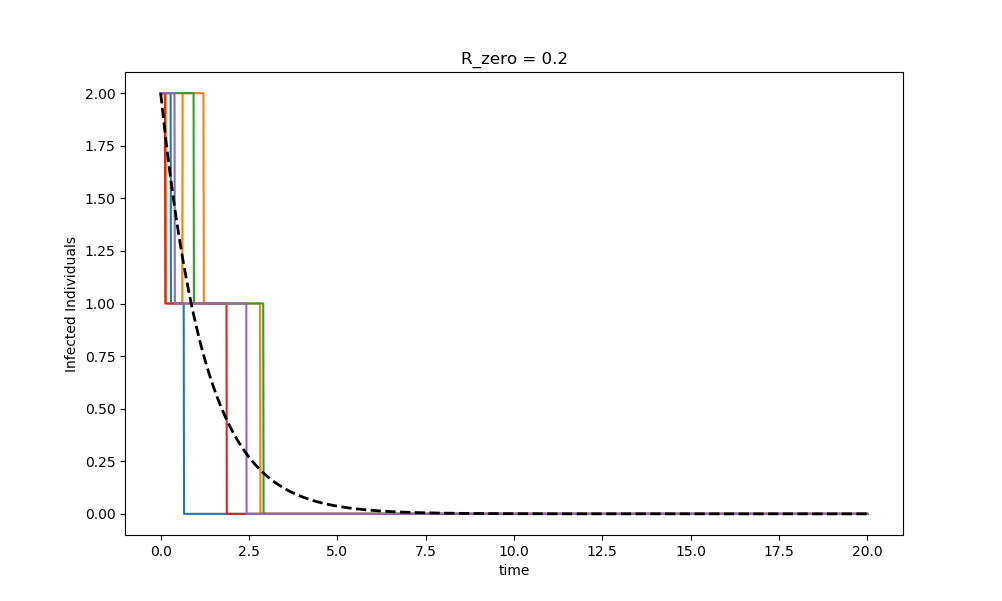
\includegraphics[width=\textwidth]{./homework/HW01.png}
%     % HW01.png: 0x0 pixel, 300dpi, 0.00x0.00 cm, bb=
%     \end{center}
% \end{frame}
%%%%%%%%%%%%%%%%%%%%%%%%%%
\begin{frame}{SIS-CTCM}
    \begin{center}
    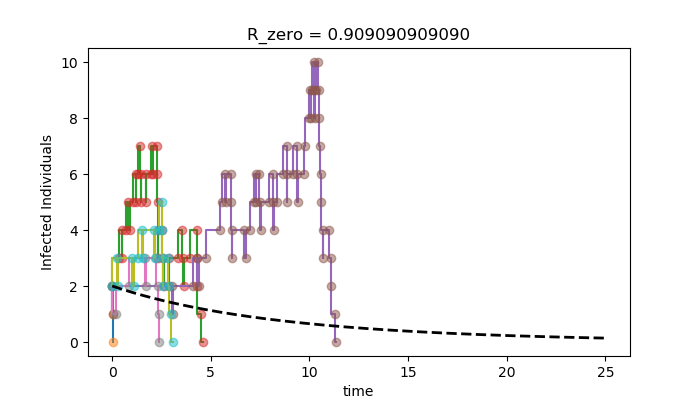
\includegraphics[width=\textwidth]{./homework/HW02.png}
    % HW01.png: 0x0 pixel, 300dpi, 0.00x0.00 cm, bb=
    \end{center}
\end{frame}
% \begin{frame}{SIS-SDE}
%     \begin{center}
%     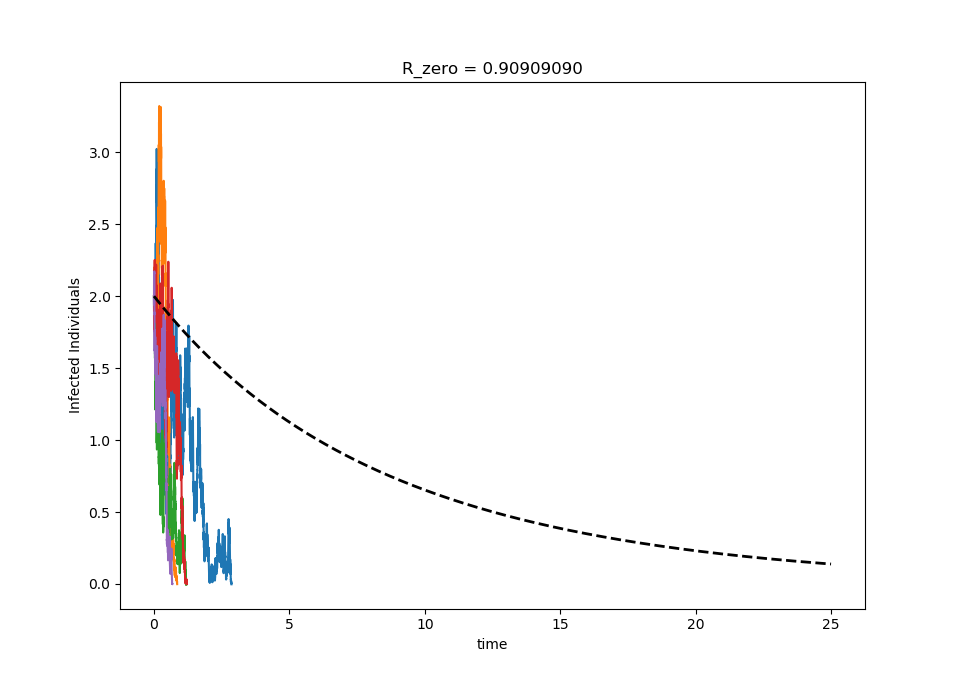
\includegraphics[width=\textwidth]{./homework/HW03.png}
%     % HW01.png: 0x0 pixel, 300dpi, 0.00x0.00 cm, bb=
%     \end{center}
% \end{frame}

    \section{Introduction}
         \begin{frame}%
     \frametitle{Analysis of an SI-SDE model}
    \begin{textblock*}{70mm}(5mm, 20mm)
        \begin{equation*}
            \begin{aligned}
                \dot{S}(t) &=
                    \Lambda - \mu S(t)
                    - \textcolor<4->{orange}{\beta}
                        S(t) I(t)
                    - \delta S(t)
                    \\
                \dot{I}(t) &=
                    \textcolor<4->{orange}{\beta}
                        S(t) I(t)
                    -(\mu + \gamma + \varepsilon) I(t)
                    \\
                \only<1-2>{
                    \dot{R}(t) &=
                        \gamma I(t)
                        - \mu R(t)
                        + \delta S(t)
                }
            \end{aligned}
        \end{equation*}
    \end{textblock*}
% %%
    \only<2-7>{
        \begin{textblock*}{50mm}(5mm, 55mm)
            \begin{tcolorbox}[%
                space to upper,%
                skin=bicolor,%
                colbacklower=black!75,%
                collower=white,%
                title={Deterministic threshold},%
                halign=center,
                valign=center,%
                bottom=2mm,%
                height=35mm%
            ]
%          \begin{graybox}
            \begin{align*}
                    \mathcal{R}_0 &=
                        \frac{\beta \Lambda}{%
                            (\mu + \gamma + \varepsilon )%
                            (\mu + \delta)%
                        }%
                    \\
                    \mathcal{R}_0  & < 1
                        \ \Rightarrow
                            \ FDE: \text{ (g.a.s)}
                    \\
                    \mathcal{R}_0  & > 1
                        \ \Rightarrow
                            \ EE: \text{\quad (g.a.s)}
                \end{align*}
            \end{tcolorbox}
         \end{textblock*}
    }
    \only<5->{
        \begin{textblock*}{42mm}(80mm, 25mm)
             \begin{tcolorbox}
                 $
                     \beta d t \rightsquigarrow
                     \beta d t + \sigma dB_t
                 $
             \end{tcolorbox}
         \end{textblock*}
    }
%     %
    \only<6->{
        \begin{textblock*}{50mm}(40mm, 40mm)
            \begin{align*}
                \dot{S}(t) &=
                    \Lambda - \mu S(t)
                    - \beta S(t) I(t)
                    - \delta S(t)
                    -
                    \hl{%
                      \sigma S(t) I(t)
                       dB_t}
                    \\
                \dot{I}(t) &=
                    \beta S(t) I(t)
                    - (\mu + \gamma + \varepsilon) I(t)
                    + \hl{\sigma S(t) I(t) dB_t}
            \end{align*}
        \end{textblock*}
    }
    \only<7>{
        \begin{textblock*}{50mm}(70mm, 55mm)
            \begin{tcolorbox}[%
                space to upper,
                skin=bicolor,
                colbacklower=black!75,
                collower=white,
                title={Stochastic threshold},
                halign=center,
                valign=center,
                bottom=2mm,
                height=35mm
            ]
                \begin{align*}
                    \mathcal{R}_0 ^ S &= \text{ ?}
                    \\
                    \mathcal{R}_0 ^ S &< 1
                    \ \Rightarrow \text{ Extinction}
                    \\
                    \mathcal{R}_0 ^ S &> 1
                    \ \Rightarrow \text{ Persistence}
                \end{align*}
            \end{tcolorbox}
        \end{textblock*}
    }
    \only<8>{
        \begin{textblock*}{105mm}(20mm, 57mm)
            \begin{tcolorbox}[title=Check:]
                \begin{bibunit}
                    \nocite{Zhang2018a}
                    \putbib
                \end{bibunit}
            \end{tcolorbox}
        \end{textblock*}
    }
\end{frame}

         \begin{frame}
    \frametitle{When apply Stochastic Models?}
    \begin{textblock*}{45mm}(3mm, 25mm)
        \begin{greenbox}{When are interested in}
            \begin{itemize}
                \item
                    Small population
                \item
                    \textcolor<2>{orange}{
                        Demographic variability
                    }
                \item
                    \textcolor<3>{orange}{
                        Environmental variability
                    }
            \end{itemize}
        \end{greenbox}
    \end{textblock*}
    \begin{textblock*}{60mm}(60mm, 25mm)
        \begin{bluebox}{
            \only<1>{
                According to
            }
            \only<2->{
                Example
            }%
        }
        \only<1>{
            \begin{bibunit}[apalike]
                \nocite{Allen2017}
                \putbib
            \end{bibunit}
        }
        \only<2->{
            Transmission,
            births, recovery,
            deaths
        }
        \only<3->{
            \tcblower
            Territorial conditions,
            aquatic: diseases
             vector, zoonotic
             Foodborne
        }
        \end{bluebox}
    \end{textblock*}
\end{frame}

         \begin{frame}
    \frametitle{Alternatives}
%%%%%%%%%%%%%%%%%%%%%%%%%%%%%%%%%%%%%%%%%%%%%%%%%%%%%%%%%%%%%%%%%%%%%%%%%%%%%%%%
    \begin{textblock*}{50mm}(3mm, 18mm)
        \begin{bluebox}{Models}
            \begin{itemize}
                \item
                    \textcolor<1>{orange}{(D/C)--TMCs}
                \item
                    \textcolor<2,3,4,5,7>{orange}{
                    \textbf<4-5,7>{%
                        Parameter perturbation
                    }
                }
                \begin{itemize}
                    \item
                        \textcolor<4>{orange}{
                            Mean reverting 
                            processes
                        }
                    \item
                        \textcolor<5>{orange}{
                            $
                                \beta_t^H \ H \in (\num{.5}, 1)
                            $
                        }
                \end{itemize}
                \item
                    \textcolor<6>{orange}{
                        Random Diff. Eq.
                    }
            \end{itemize}
        \end{bluebox}
    \end{textblock*}
% %%%%%%%%%%%%%%%%%%%%%%%%%%%%%%%%%%%%%%%%%%%%%%%%%%%%%%%%%%%%%%%%%%%%%%%%%%%%%%%%
    \begin{textblock*}{72mm}(55mm, 18mm)
       \begin{graybox}
            {%
                \only<1>{%
                    $\mathbf{MC}
                    +\mathbf{ME}$
                    $\to$ $SDE$%
                }%
                \only<2>{%
                    $\varphi dt \rightsquigarrow \varphi dt+ \sigma dB_t$%
                }%
                \only<3>{%
                    $\varphi dt \rightsquigarrow \varphi dt+F(x)dB_t$%
                }%
                \only<4>{%
                    $d
                        \varphi_t =
                        (\varphi_e - \varphi_t) dt
                        + \sigma_\varphi dB_t
                    $%
                }%
                \only<5>{
                    Fractiona BM.: long range memory.
                }
                \only<6>{%
                    parameters as r.v.
                }%
                \only<7>{%
                    $\varphi dt \rightsquigarrow \varphi dt+ \sigma dB_t$%
                }%
            }%Block titles
            \only<1>{
                \begin{bibunit}[abbrv]
                    \nocite{Allen2017}
                    \putbib
                \end{bibunit}
            }
            \only<2,7>{
                \begin{bibunit}[apalike]
                    \nocite{Gray2011}
                    \putbib
                \end{bibunit}
            }
            \only<3>{
                \begin{bibunit}[apalike]
                    \nocite{Schurz2015}
                    \putbib
                \end{bibunit}
            }
            \only<4>{
                \begin{bibunit}[apalike]
                    \nocite{Allen2016}
                    \putbib
                \end{bibunit}
            }
            \only<5>{
                \begin{bibunit}[apalike]
                    \nocite{Ma2017}
                    \putbib
                \end{bibunit}
            }
            \only<6>{
                \begin{bibunit}[apalike]
                    \nocite{Chen-Charpentier2015}
                    \putbib
                \end{bibunit}
            }
        \end{graybox}
   \end{textblock*}
   \begin{textblock*}{50mm}(3mm, 68mm)
        \begin{greenbox}{Tools}
            \begin{list}{$\bullet$}{}
                \item
                    Gillespie
                \item
                    \small{Kloeden}-\normalsize{Methods}
                \item
                    Hermite-PC
            \end{list}
        \end{greenbox}
    \end{textblock*}
\end{frame}

         \begin{frame}
    \frametitle{Objetivo}
    \begin{textblock*}{80mm}(25mm, 40mm)
            \begin{yellowbox}{%
                To illustrate ideas 
                $
                    \varphi dt 
                    \rightsquigarrow 
                    \varphi dt 
                    + 
                    \sigma dB_t
                $
            }
                \begin{list}{$\bullet$}{}
                    \item
                        Modelling
                    \item
                        Analysis and simulation 
                    \item
                        Perspectives
                \end{list}
            \end{yellowbox}
    \end{textblock*}
\end{frame}
%         %
        \begin{frame}{Esquema de Charla}
            \setbeamertemplate{section in toc}[sections numbered]
            \tableofcontents[hideallsubsections]
        \end{frame}
    \section{Perturbaci\'on con MB}
         \begin{frame}
    \frametitle{Modelo de jugete}
    \begin{textblock*}{70mm}(1mm, 15mm)
        \only<1-9>{
            \begin{bluebox}{}
                \begin{align*}
                    \dfrac{dS(t)}{dt} &= 
                        \mu N - \beta S(t) I(t) + \gamma I(t) - \mu S(t),
                    \\
                    \dfrac{I(t)}{dt} &=
                        \beta S(t) I(t) - (\mu + \gamma) I(t),
                    \\
                    R_0 ^ D &= 
                        \frac{\beta N}{\mu + \gamma},
                    \\
                    \only<1>{
                        R_0 ^ D  &< 1
                        \ \Rightarrow
                            \lim_{t \to \infty}
                                I(t) = 0
                        \\
                        R_0 ^ D  &> 1
                        \ \Rightarrow
                            \lim_{t \to \infty}
                                I(t) = 
                                N
                                \left(
                                    1 -
                                    \frac{1}{R_0 ^ D}
                                \right)
                    }
                \end{align*}
            \end{bluebox}
        }
        \only<2-7>{
            $
                d I(t) = 
                    \left[ 
                        \beta S(t) I(t) - (\mu + \gamma) I(t)
                    \right] dt
            $
        }
        \only<7-8>{
            \begin{align*}
                dS(t) &= 
                    [\mu N - \beta S(t) I(t) + \gamma I(t) - \mu S(t)] dt
                    - \sigma S(t)I(t)dB_t
                \\
                dI(t) &=
                    [\beta S(t) I(t) - (\mu + \gamma) I(t)]
                    dt
                    + \sigma S(t)I(t)  
                    dB_t
            \end{align*}
        }
        \only<9>{
            \begin{align*}
                N &= S(t)+I(t) = \text{cte.}
                \\
                dI(t) &= 
                    I(t)
                    \left(
                        [
                            \beta (N - I(t))
                            -\mu - \gamma
                        ]
                    \right)
                     dt
                    -\sigma (N-I(t))
                    dB_t
            \end{align*}
        }
    \end{textblock*}
    \only<6>{
        \begin{textblock*}{47mm}(80mm, 55mm)
             \begin{tcolorbox}
                 \begin{align*}
                    \beta d t  \rightsquigarrow & 
                    \underbrace{
                        \beta dt + \sigma dB_t
                    }_{:= \tilde{\beta} dt}
                    \\
                    \mathbb{E} [\tilde{\beta} dt] 
                        & = \beta dt
                    \\
                    \mathbb{V}ar [\tilde{\beta} dt]
                        & = \sigma^2 dt 
                        \xrightarrow{dt \to 0}
                        0 
                 \end{align*}
             \end{tcolorbox}
         \end{textblock*}
    }
%%%%%%%%%%%%%%%%%%%%%%%%%%%%%%%%%%%%%%%%%%%%%%%%%%%%%%%%%%%%%%%%%%%%%%%%%%%%%%%%
    \begin{textblock*}{60mm}(70mm, 15mm)
        \only<2-6>{
            \begin{itemize}
                \item<3-6>
                    $
                        (
                            \Omega,
                            \mathcal{F},
                            \{\mathcal{F}\}_{t \geq 0},
                            \mathbb{P}
                        )
                   $,
                \item<4-6>
                    $B_t$ M.B.
                \item<5-6>
                    $\beta S(t)I(t) dt$ 
                    \\
                    nuevas infecciones en $[t,t+dt)$
                \item<6>
                    $\beta dt$, contactos potencialmente infecciosos
            \end{itemize}
        }
    \end{textblock*}
  \end{frame}
    \section{Solution properties}
         \begin{frame}
    \frametitle{Existence and uniqueness of a positive solution}
    \begin{textblock*}{60mm}(10mm, 25mm)
        \begin{yellowbox}{Theorem}
            \begin{list}{$\bullet$}{}
                \item
                    $ \forall I(0) \in (0, N)$
            \end{list}
            \tcblower
             $! \exists$
             \textbf{global positive invariant solution % 
             $I_t$} 
            %
            $$
                \probX{I(t) \in (0, N) \forall t \geq 0} = 1.
            $$
        \end{yellowbox}
    \end{textblock*}
%%%%%%%%%%%%%%%%%%%%%%%%%%%%%%%%%%%%%%%%%%%%%%%%%%%%%%%%%%%%%%%%%%%%%
    \begin{textblock*}{60mm}(65mm, 25mm)
        \begin{align*}
            dI(t) &= 
                I(t)
                 \left\{
                     [
                         \beta (N - I(t))
                         -\mu - \gamma
                     ]
                     dt
                 \right.
                 \\
                  &+
                 \left.
                     \sigma (N-I(t))
                     dB_t
                 \right\}
                 %\tag{\star}
        \end{align*}
    \end{textblock*}
\end{frame}
%%%%%%%%%%%%%%%%%%%%%%%%%%%%%%%%%%%%%%%%%%%%%%%%%%%%%%%%%%%%%%%%%%%%%%%%%%%%%%%%
\begin{frame}
     \frametitle{Extinction by noise}
        \begin{textblock*}{65mm}(0mm, 25mm)
            \begin{yellowbox}{Theorem}
                \begin{list}{$\bullet$}{}
                    \item
                        $
                            \displaystyle
                            \sigma ^ 2 
                            >
                            \max
                            \left\{
                                \frac{\beta}{N},
                                \frac{\beta^2}{2(\mu + \gamma)}
                            \right\}
                        $
                \end{list}
                \tcblower
                for all $I(0)\in (0, N)$ the solution to SDE($\star$)
                satisfies
                $$
                    \limsup_{t \to \infty} 
                        \frac{1}{t} \log I(t)
                        \leq
                        \underbrace{
                        -\mu - \gamma 
                        + \frac{\beta^2}{2 \sigma ^ 2}
                        }_{<0}
                $$
            \end{yellowbox}
        \end{textblock*}
\end{frame}
%%%%%%%%%%%%%%%%%%%%%%%%%%%%%%%%%%%%%%%%%%%%%%%%%%%%%%%%%%%%%%%%%%%%%%%%%%%%%%%%
\begin{frame}
    \frametitle{Simulación: Extinción por ruido ambiental}
    \begin{figure}[h!]
        \centering
        \includegraphics[width=1.01\textwidth, keepaspectratio]%
        {./Figures/IStochastiSIS00.png}
        %\caption{Extinción}
    \end{figure}
\end{frame}

    \section{%
        Trheshold: %
        $   
            R_0 ^ S := 
                R_0 ^ D 
                -%
                f(\sigma, \cdot)
        $
    }%
         \begin{frame}
    \frametitle{Extinción}
        \begin{textblock*}{65mm}(1mm, 20mm)
            \begin{yellowbox}{Theorem (Extinction)}
                \begin{list}{$\bullet$}{}
                    \item
                        $
                            \displaystyle
                            R_0 ^ S := R_0 ^D
                            - \frac{\sigma ^ 2}{2(\mu + \gamma)} < 1
                        $
                    \item
                        $
                            \displaystyle
                            \sigma^2 \leq \frac{\beta}{N}
                        $
                \end{list}
                \tcblower
                for all $I(0)\in (0, N)$
                \begin{align*}
                    &\limsup_{t \to \infty} 
                    \frac{1}{t} \log I(t)
                        \leq
                        \kappa,  \quad c.s.
                    \\
                        &\kappa :=
                        \beta N - \mu - \gamma 
                        - \frac{\sigma^2 N^2}{2 \sigma ^ 2}
                        <0 
                \end{align*}
            \end{yellowbox}
        \end{textblock*}
        \begin{textblock*}{62mm}(65mm, 25mm)
            \begin{align*}
                dI(t) &= 
                    I(t)
                    \left\{
                        [
                            \beta (N - I(t))
                            -\mu - \gamma
                        ]
                        dt
                    \right.
                    \\
                     &+
                    \left.
                        \sigma (N-I(t))
                        dB_t
                    \right\}
                    \tag{$\star$}
            \end{align*}
        \end{textblock*}
\end{frame}
\begin{frame}
    \frametitle{Extinction by a threshold condition}
    \begin{figure}[h!]
        \centering
        \includegraphics[width=1.01\textwidth, keepaspectratio]%
        {./Figures/IStochastiSIS01.png}
        %\caption{Extinción}
    \end{figure}
\end{frame}
%%%%%%%%%%%%%%%%%%%%%%%%%%%%%%%%%%%%%%%%%%%%%%%%%%%%%%%%%%%%%%%%%%%%%%%%%%%%%%%%

         \begin{frame}
    \frametitle{Persistence}
        \begin{textblock*}{62mm}(1mm, 25mm)
            \begin{yellowbox}{Theorem (persistence)}
                \begin{list}{$\bullet$}{}
                    \item
                        $
                            \displaystyle
                            R_0 ^ S := R_0 ^D
                            - \frac{\sigma ^ 2}{2(\mu + \gamma)} > 1
                        $
                \end{list}
                 \tcblower
                 para toda $I(0)\in (0, N)$
                \begin{align*}
                    \limsup_{t \to \infty} 
                        \frac{1}{t} \log I(t)
                        &
                        \geq
                        \varepsilon,
                    \\
                    \liminf_{t \to \infty}
                        \frac{1}{t} \log I(t)
                        &
                        \leq
                        \varepsilon,  \quad c.s.
                \end{align*}
            \scalebox{0.8}{
                $
                    \varepsilon =
                    \frac{1}{\sigma^2}
                    \left(
                        \sqrt{
                            \beta^2 - 2 \sigma^2 (\mu + \gamma)
                            -(\beta - \sigma^2 N)
                        }
                    \right)
               $
            }
            \end{yellowbox}
        \end{textblock*}
%%%%%%%%%%%%%%%%%%%%%%%%%%%%%%%%%%%%%%%%%%%%%%%%%%%%%%%%%%%%%%%%%%%%%%%%%%%%%%%
         \begin{textblock*}{62mm}(65mm, 25mm)
            \begin{align*}
                dI(t) &= 
                    I(t)
                    \left\{
                        [
                            \beta (N - I(t))
                            -\mu - \gamma
                        ]
                        dt
                    \right.
                    \\
                     &+
                    \left.
                        \sigma (N-I(t))
                        dB_t
                    \right\}
                    \tag{$\star$}
            \end{align*}
           \begin{bluebox}{$R_0 ^ D: \beta N /(\mu + \gamma)$}
                \begin{align*}
                    R_0 ^ D & < 1
                    \ \Rightarrow
                        \lim_{t \to \infty}
                            I(t) = 0
                    \\
                    R_0 ^ D & > 1
                    \ \Rightarrow
                        \lim_{t \to \infty}
                            I(t) = 
                            N
                            \left(
                                1 -
                                \frac{1}{R_0 ^ D}
                            \right)
                \end{align*}
            \end{bluebox}
         \end{textblock*}
\end{frame}
\begin{frame}
    \frametitle{Simulation: Persistence)}
    \begin{figure}[h!]
        \centering
        \includegraphics[width=1.01\textwidth, keepaspectratio]%
        {./Figures/IStochastiSIS02.png}
        %\caption{Extinción}
    \end{figure}
\end{frame}

         \begin{frame}
    \begin{textblock*}{60mm}(1mm, 25mm)
        \frametitle{Stationary distribution}
        \begin{greenbox}{Stationary distribution}
            \begin{list}{$\bullet$}{}
                \item
                    $
                        P_{I_0,t}(A)
                        = \probX{I(t)\in A}
                    $,
                    \\
                    $A \in \mathcal{B}((0, N))$
                \item
                    $
                        \displaystyle
                        \lim_{t \to \infty}
                        P_{I_0,t}(\cdot)
                        = \mathbb{P}_{\infty}(\cdot)
                    $ 
                    \\
                    in distribution.
            \end{list}
        \end{greenbox}
    \end{textblock*}
    \begin{textblock*}{60mm}(61mm, 20mm)
        \only<3>{
            \includegraphics[width=\textwidth, keepaspectratio]%
            {Figures/histo_sigma_1.png}
        }
        \only<4>{
            \includegraphics[width=\textwidth, keepaspectratio]%
            {Figures/histo_sigma_2.png}
        }
    \end{textblock*}
\end{frame}

     \section{Perspectives and fina comments}
         \begin{frame}[plain]
    \frametitle{}
    \only<1>{
        \begin{bibunit}
            \nocite{Jerez2018,Acuna-Zegarra2018}
            \putbib
        \end{bibunit}
    }
    \only<2>{
        \begin{bibunit}
            \nocite{Diaz-Infante2017a}
            \putbib
        \end{bibunit}
    }
\end{frame}
%%%%%%%%%%%%%%%%%%%%%%%%%%%%%%%%%%%%%%%%%%%%%%%%%%%%%%%%%%%%%%%%%%%%%%%%%%%%%%%%
\begin{frame}
    \frametitle{Perspectives}
        \begin{textblock*}{50mm}(3mm, 18mm)
            \begin{bluebox}{Modelos}
                \begin{itemize}
                        \item
                            \textcolor<1>{orange}{
                                Mean reverting processes
                            }
                        \item
                            \textcolor<2>{orange}{
                                $
                                    \beta_t^H \ H \in (\num{.5}, 1)
                                $
                            }
                        \item
                            \textcolor<3>{orange}{
                                Random Diff. Eq.
                            }
                        \item
                            Random Dynamical Systems
                \end{itemize}
            \end{bluebox}
        \end{textblock*}
%%%%%%%%%%%%%%%%%%%%%%%%%%%%%%%%%%%%%%%%%%%%%%%%%%%%%%%%%%%%%%%%%%%%%%%%%%%%%%%%
        \begin{textblock*}{72mm}(55mm, 18mm)
           \begin{graybox}{
                \only<1>{%
                    $d
                        \varphi_t =
                        (\varphi_e - \varphi_t) dt
                        + \sigma_\varphi dB_t
                    $%
                }%
                \only<2>{
                    Long time memory: fBM
                }
                \only<3>{%
                    Parameters as r.v
                }
            }%
                \only<1>{
                    \begin{bibunit}[apalike]
                        \nocite{Allen2016}
                        \putbib
                    \end{bibunit}
                }
                \only<2>{
                    \begin{bibunit}[apalike]
                        \nocite{Ma2017}
                        \putbib
                    \end{bibunit}
                }
                \only<3>{
                    \begin{bibunit}[apalike]
                        \nocite{Chen-Charpentier2015}
                        \putbib
                    \end{bibunit}
                }
          \end{graybox}
       \end{textblock*}
\end{frame}
%%%%%%%%%%%%%%%%%%%%%%%%%%%%%%%%%%%%%%%%%%%%%%%%%%%%%%%%%%%%%%%%%%%%%%%%%%%%%%%%
\begin{frame}
    \frametitle{The Bibles:}
    \only<1>{
        \begin{bibunit}
            \nocite{Freidlin1998,Khasminskii}
            \putbib
        \end{bibunit}
    }
    \only<2>{
        \begin{bibunit}
            \nocite{Kloeden1995, Kloeden2017}
            \putbib
        \end{bibunit}
    }
\end{frame}
%%%%%%%%%%%%%%%%%%%%%%%%%%%%%%%%%%%%%%%%%%%%%%%%%%%%%%%%%%%%%%%%%%%%%%%%%%%%%%%%%
\begin{frame}
    \frametitle{Coments about the OCM}
    \begin{textblock*}{72mm}(15mm, 18mm)
        \begin{graybox}{About the policies}
            \begin{itemize}
                \item
                 $u = u(t)$, possible improvement
                \item
                 $u = (x)$, or $u = u(t,x)$ 
                \item
                    uncertinity
            \end{itemize}
        Tool: Dynamical Programing-HJB, MDP .
        \end{graybox}    
    \end{textblock*}
\end{frame}
%%%%%%%%%%%%%%%%%%%%%%%%%%%%%%%%%%%%%%%%%%%%%%%%%%%%%%%%%%%%%%%%%%%%%%%%%%%%%
\begin{frame}
    \frametitle{Towards Stochastic Control}
    \begin{textblock*}{72mm}(10mm, 10mm)
        \begin{graybox}{About the policies}
            \begin{align*}
                &
                \min_{u\in \mathcal{U}} \EX{\int_0^T f(t,x,u)}
                \\
                s.t.& 
                    \qquad dx_t = a(t,x,u)dt
                        + b(t,x,u) dw_t
            \end{align*}
        Tools: Dynamic Programing - HJB, MDP, Viscosity Solution,
        \end{graybox}    
    \end{textblock*}
    \only<2>{
        \begin{textblock*}{60mm}(10mm, 60mm)
            \begin{bibunit}
                \nocite{stochastic_control_sis}           
                \putbib
            \end{bibunit}
        \end{textblock*}
    }
    \only<3>{
        \begin{textblock*}{60mm}(10mm, 60mm)
            \begin{bibunit}
                \nocite{winner_chaos}           
                \putbib
            \end{bibunit}
        \end{textblock*}
    }
\end{frame}
%%%%%%%%%%%%%%%%%%%%%%%%%%%%%%%%%%%%%%%%%%%%%%%%%%%%%%%%%%%%%%%%%%%%%%
\begin{frame}
    \frametitle{The END}
    \begin{graybox}{Code: \texttt{*.tex, *.py}}
        \begin{center}
            \href{
               https://github.com/SaulDiazInfante/Modelling-Simulation-with-SDE%
            }%
            {https://github.com/SaulDiazInfante/Modelling-Simulation-with-SDE}
        \end{center}
        \only<2>{
            \begin{center}
                \Huge{Gracias!!!}
            \end{center}
        }
    \end{graybox}
\end{frame}
\end{document}